\documentclass[prl, 11 pt]{revtex4-2}
\linespread{0.9} % Adjust the value as needed; default is 1.0
\setlength{\parindent}{0pt}  % No indentation globally

\usepackage{graphicx}
\usepackage{color}
\usepackage{latexsym,amsmath}
\usepackage{amsfonts}
\usepackage{caption}
\usepackage{siunitx}
\usepackage{physics}


\definecolor{linkcolor}{rgb}{1.0,0.647,0.0} %hyperlink
\usepackage[pdftex,colorlinks=true, pdfstartview=FitV, linkcolor= linkcolor, citecolor= linkcolor, urlcolor= linkcolor, hyperindex=true,hyperfigures=true]{hyperref} %hyperlink%

\usepackage{enumitem}
\setlist[itemize]{leftmargin=*}


\setcounter{secnumdepth}{2}

\renewcommand{\thesection}{\arabic{section}}
\renewcommand{\theequation}{\thesection.\arabic{equation}}

\makeatletter
\@addtoreset{equation}{section} % Reset equation counter at each section
\makeatother

\begin{document}

\title{Quantum Optics and Laser - Homework}

\author{Calandra Buonaura Lorenzo}

\date{\today}

\maketitle

\section{Phase uncertainty for coherent states}
\subsection{Problem statement}
In the hypothesis of $|\alpha|$ significantly larger than unity, discuss the general expression for the phase uncertainty as $\sqrt{(\Delta \phi)^2}$ as a function of the average photon number. Discuss the two following cases in which a single mode with $\lambda = 633$~nm may be found:
\begin{enumerate}
    \item the coherent state with $\alpha = 4 + i3$.
    \item a coherent beam with power of $3$~pW.
\end{enumerate}

\subsection{Solution}
The problem concerns coherent states, which are quantum states of the electromagnetic field that most closely resemble classical light. The normalized coherent state is defined as:
%
\begin{equation}
    \label{eq:coherent_state_def}
    \ket{\alpha} = e^{-\frac{|\alpha|^2}{2}}\;\sum_{n=0}^\infty\frac{\alpha^n}{\sqrt{n!}}\ket{n}
\end{equation}
%
where $\alpha$ is a complex number representing the amplitude of the coherent state, and $\ket{n}$ denotes the number state (or Fock state) with $n$ photons. Coherent states are eigenstates of the annihilation operator $\hat{a}$ and follow the relation:
%
\begin{equation}
    \label{eq:a_eigenstates}
    \hat{a}\ket{\alpha} =\alpha\ket{\alpha}
\end{equation}
%
Thus, remembering the definition of the number operator $\hat{n} = \hat{a^\dagger} \hat{a}$, we can compute the average photon number $\langle \hat{n} \rangle$ for a coherent state as:
%
\begin{equation}
    \label{eq:avg_photon_number}
    \langle \hat{n} \rangle = \langle \alpha | \hat{a}^\dagger \hat{a} | \alpha \rangle = |\alpha|^2,  
\end{equation}
%
where \( \hat{a}^\dagger \) and \( \hat{a} \) are the creation and annihilation operators, respectively. Now, the probability of finding a system in the number state $|n\rangle$ when it is in a coherent state $|\alpha\rangle$ is given by the square of the probability amplitude $\langle n|\alpha\rangle$:
%
\begin{equation}
    P(n) = |\langle n|\alpha \rangle|^2 = e^{-\left|\alpha\right|^2} \frac{|\alpha|^{2n}}{n!} = e^{-\bar{n}^2} \frac{\bar{n}^{2n}}{n!}
\end{equation}
%
which is a Poisson distribution depending on the mean photon number as parameter.

We are interested instead in the phase distribution, which for a coherent state $\ket{\alpha}$ with $\alpha = |\alpha|e^{i\theta}$ is given by:
%
\begin{equation}
    P(\phi) = \frac{1}{2\pi} |\langle \phi|\alpha \rangle|^2= \frac{1}{2\pi} e^{-|\alpha|^2} \left|\sum_{n=0}^{\infty} \frac{|\alpha|^n}{\sqrt{n!}} e^{in(\phi-\theta)} \right|^2
\end{equation}
%
In the approximation of large $|\alpha|$ (which means also large $|\alpha|^2$), we can approximate the phase distribution $P(\phi)$ to a Gaussian distribution, obtaining an approximate form:
%
\begin{equation}
    \label{eq:p_phi}
    P(\phi) \approx \frac{\sqrt{2}|\alpha|}{\sqrt{\pi}} e^{-(2|\alpha|^2(\phi - \theta)^2)}
\end{equation}
%
Comparing this expression to the general expression of a Gaussian distribution we get that the standard deviation of the distribution, which represents the phase uncertainty, is related to the average photon number:
%
\begin{equation}
    \label{eq:delta_phi}
    \Delta\phi = \frac{1}{2|\alpha|}
\end{equation}

We can now apply Equation~\eqref{eq:delta_phi} to the two cases requested:
\begin{enumerate}
    \item \textbf{Coherent state with $\alpha = 4 + i3$}
    
    For $\alpha = 4 + i3$, the amplitude $|\alpha|$ is:
    $$
        |\alpha| = \sqrt{\Re(\alpha)^2 + \Im(\alpha)^2} = \sqrt{4^2 + 3^2} = 5.
    $$
        
    Thus, using Equation~\eqref{eq:avg_photon_number} for the average photon number, the phase uncertainty (in the large $|\alpha|$ limit) is:
    $$
        \Delta \phi = \frac{1}{2\sqrt{\langle n \rangle}} = \frac{1}{2\sqrt{|\alpha|^2}} = \frac{1}{2|\alpha|} = \frac{1}{10} = 0.1~\si{\hertz}
    $$

    \item \textbf{Coherent beam with power of 3 pW}

    A coherent beam is a beam of light where the wavefronts of the photons are in phase or maintain a consistent phase relationship over time and space; in this case, the average photon number $\langle n \rangle$ can be computed as:
    %
    \begin{equation}
        \label{eq:avg_n_ex1.2}
        \langle n \rangle = \Phi \:T
    \end{equation}
    %
    where $\Phi$ is the mean photon flux and $T$ is the time duration of the operation. The flux, assumed to be continuous, can be simply obtained as:
    %   
    \begin{equation}
        \label{eq:flux}
        \Phi = P\; \frac{\lambda}{hc}
    \end{equation}
    where $h$ is Planck’s constant, $c$ is the speed of light, $P$ is the beam's power, and $\lambda$ is the peak wavelength. We have all the needed quantity for computing $\langle n \rangle$ except for $T$: nevertheless, we can suppose that we shine the beam for a fixed amount of time, like $T = 1~\si{\second}$. With this approximation, we can compute the average number of photons using Equation~\eqref{eq:avg_n_ex1.2}:
    %
    $$
        \langle n \rangle = \Phi \:T = P\; \frac{\lambda}{hc} \:T \approx 9.56 \times 10^6
    $$
    %
    Finally, we get that the phase uncertainty is:
    $$
        \Delta \phi = \frac{1}{2\sqrt{\langle n \rangle}} = 1.62 \times 10^{-4}~\si{\hertz}
    $$
\end{enumerate}

Based on these results, we can observe that the phase uncertainty $\Delta \phi$ decreases as the average photon number $\langle n \rangle$ increases. In particular, in the first case, the average photon number is relatively small ($\langle n \rangle = 25$), leading to a moderate phase uncertainty of $\Delta \phi = 0.1~\si{\hertz}$: this value reflects the limited precision achievable when the average photon count is low, as in the case of a specific Fock state. On the other hand, when considering a laser like in the second case, we get an average photon number of approximately $\langle n \rangle = 9.56 \times 10^6$, which makes the phase uncertainty significantly smaller, $\Delta \phi = 1.62 \times 10^{-4}~\si{\hertz}$, showcasing the precision enhancement possible with powerful and coherent light sources.

%%%%%%%%%%%%%%%%%%%%%%%%%%%%%%%%%%%%%%%%%%%%%%%%%%%%%%%%%%%%%%%%%%%%%%%%%

\newpage
\section{Absorption of a photon in number states}
\subsection{Problem statement}
Consider the superposition of the vacuum and 30-photon number state:
%
\begin{equation*}
    \ket{\psi} = \frac{\ket{0} + \ket{30}}{\sqrt{2}}.
\end{equation*}
%
\begin{enumerate}
    \item Calculate the average photon number for this state.
    \item Now, the annihilation operator is applied to the state, so a single photon is absorbed. Calculate the new value for the average photon number.
    \item Analyze the two results and discuss the meaning of the average photon number.
\end{enumerate}

\subsection{Solution}
For this problem we are considering a quantum state which is the superposition of two Fock's state, the vacuum $\ket{0}$ and the 30-photon state $\ket{30}$; the state $\ket{\psi}$ is already normalized as it's divided by $\sqrt{2}$, which accounts for the equal probability of the two states.

\begin{enumerate}
    \item The first request of the assignment is computing the average photon number $\langle n \rangle$, which is the expectation value of the number operator over the state $\psi$:
    $$
        \langle n \rangle = \langle \psi | n | \psi \rangle = \left\langle\frac{\bra{0} + \bra{30}}{\sqrt{2}} \right| \hat{n} \left| \frac{\ket{0} + \ket{30}}{\sqrt{2}}\right\rangle
    $$
    Expanding the terms we get:
    $$
        \langle n \rangle = \frac{1}{2} \Big( \langle 0|\hat{n}|0\rangle + \langle 0|\hat{n}|30\rangle + \langle 30|\hat{n}|0\rangle + \langle  30|\hat{n}|30\rangle \Big)
    $$
    Now, in order to proceed, we must remember how the number operator works when applied to a Fock state $\ket{n}$:
    \begin{equation}
        \label{eq:n_op}
        \hat{n}\ket{n} = n\ket{n}.
    \end{equation}
    Using this property and the orthonormality of the Fock's states, we simplify the terms:
    \begin{align*}
        \langle 0|\hat{n}|0\rangle & = 0, \\
        \langle 0|\hat{n}|30\rangle & = 0, \\
        \langle 30|\hat{n}|0\rangle & = 0, \\
        \langle 30|\hat{n}|30\rangle & = 30.
    \end{align*}
    Substituting back, we find:
    $$
        \langle n \rangle = \frac{1}{2} \Big( 0 + 0 + 0 + 30 \Big) = \frac{30}{2} = 15.
    $$
    %
    \item The second request of the assignment is calculating again the average photon number $\langle n \rangle$ for the state $\ket{\psi}$, but after that the annihilation operator is applied to it. First we must compute the new state $\hat{a}\ket{\psi}$, remembering how the annihilation operator acts on Fock's states:
    \begin{equation}
        \label{eq:a_op}
        \hat{a}\ket{n} = \sqrt{n}\ket{n-1}
    \end{equation}
    Using this property, we get:
    $$
        \hat{a}\ket{\psi} = \hat{a} \left(\frac{\ket{0} + \ket{30}}{\sqrt{2}}\right) = \frac{1}{\sqrt{2}}(\hat{a}\ket{0} + \hat{a}\ket{30}) = \frac{1}{\sqrt{2}}(0 + \sqrt{30}\ket{29}) = \sqrt{15}\ket{29}
    $$
    Nevertheless, this state is not normalized, due to the factor in front: before computing the average photon number, we need to normalize again, simply removing the factor, leaving with:
    $$
        \hat{a}\ket{\psi} = \ket{29}
    $$
    Then, using Equation~\eqref{eq:n_op}, we can compute the average photon number:
    $$
        \langle n \rangle = \bra{29} \hat{n} \ket{29} = 29
    $$
    %
    \item  In the first case, the average photon number is 15. This value arises from the equal superposition of two Fock states, the vacuum state $\ket{0}$ with no photons and the $\ket{30}$ state with 30 photons: since both states contribute equally, the average photon number is simply the arithmetic mean of the average occupation of the two states (0 and 30 photons, respectively). In the second case, the annihilation operator reduces the photon number in each Fock state by one. Since $\ket{0}$ vanishes under $\hat{a}$, only the $\ket{30}$ term contributes, reducing to $\ket{29}$. This results in a definite photon number of 29.

    These results illustrate how the average photon number depends on the quantum state's composition. For a superposition, \(\langle n \rangle\) is the expectation value, representing the mean contribution of all photon number states. After applying the annihilation operator, the state collapses to a single Fock state, where \(\langle n \rangle\) directly equals the photon number of the new state. This demonstrates the probabilistic nature of quantum mechanics and the operator's effect, which reduces photon numbers and alters the photon statistics, removing contributions from parts of the superposition.

\end{enumerate}

%%%%%%%%%%%%%%%%%%%%%%%%%%%%%%%%%%%%%%%%%%%%%%%%%%%%%%%%%%%%%%%%%%%%%%%%%

\newpage
\section{Nd:YAG optical amplifier}
\subsection{Problem statement}
An amplifier based on the 4-level system exploiting a Nd:YAG rod (diameter $4$~mm, length $50$~mm) as the active medium has the following characteristics:
$\sigma_0 = 2.8 \times 10^{-19}~\si{cm^{2}}$, central gain wavelength $\lambda = 1064$~nm, $\tau = 230~\si{\micro\second}$, volume concentration in the crystal of Nd ions: $1.1\%$. When the pumping system is activated, the amplifier has a $\gamma_0 = 2~\si{cm^{-1}}$.
\begin{enumerate}
    \item Calculate the pumping rate $W = R_2$ considering $R_1 \approx 0$ and the actual population inversion value.
    \item Consider pumping at $\lambda = 808$~nm. What is the pumping power necessary to obtain the gain?
    \item Calculate the saturation intensity of the amplifier and plot the saturated gain as a function of the incident flux, expressed in beam intensity.
    \item What is the total gain of the entire rod in the small signal regime?
\end{enumerate}

\subsection{Solution}

This problem involves an amplifier based on a 4-level laser pumping scheme, as depicted in Figure~\ref{fig:four_level_scheme}. In this arrangement, level 0 is the ground state and level 1, which is a short-lived state, lies above the ground state; in thermal equilibrium, level 1 is not populated (or at least it has a very small population). Pumping is accomplished by making use of an energy level 3, which lies above the long-lived state 2; again, the 3 $\rightarrow$ 2 transition has a short lifetime, so that there is little population accumulation in level 3. Thus, four energy levels are involved in the process, but the optical interaction of interest takes place between levels 2 and 1. After this brief introduction, we can start solving the request of the problem:

%
\begin{figure}[!b]
    \centering
    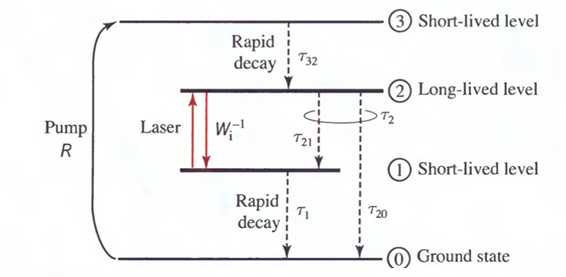
\includegraphics[width=0.5\linewidth]{Images/four_level_scheme.png}
    \caption{Four levels pumping scheme.}
    \label{fig:four_level_scheme}
\end{figure}
%

\begin{enumerate}
    \item For the first question, we must consider $R_1 \approx 0$ and compute the pumping rate $W = R_2$. This can be easily obtained from the relation that defines the steady-state population difference, $\Delta N$, between the upper laser level (2) and the lower level (1), which can be determined using the relevant rate equations. Here, level 2 is considered instead of level 3 due to the rapid decay, which can effectively be regarded as instantaneous, making it reasonable to treat the pumping process as if it directly populates level 2. The steady-state population, in absence of non-radiative decay component and with $R_1 \approx 0$, is defined as:
    %
    \begin{equation}
        \label{eq:delta_N}
        \Delta N \approx R_2\tau
    \end{equation}
    %
    where $\tau$ is the fluorescence lifetime. Thus, in order to compute $R_2$ we must find another way of computing $\Delta N$; in order to do so, we can leverage the fact that this is an amplifier in the small-signal regime. Thus, we can express the dependency of $\Delta N$ from $\gamma_0$ (small-signal gain coefficient) and $\sigma_0$ (cross-section for stimulated emission) as:
    %
    \begin{equation}
        \label{eq:gamma_0}
        \gamma_0 = \Delta N \sigma_0
    \end{equation}
    %
    From Equation~\eqref{eq:gamma_0} we get:
    $$
        \Delta N = 7.14 \times 10^{18}~\text{ions}/\si{\cm^{3}}
    $$
    Thus, inverting Equation~\eqref{eq:delta_N}, we get:
    $$
        W = R_2 = \frac{\Delta N}{\tau} = 3.10 \times 10^{22}~\text{ions}/\si{\second}\;\si{\cm^3}
    $$
    where the pumping rate is expressed as events per second per unit volume.
    \item The second request asks to compute the pumping power necessary to obtain $\gamma_0$ at a fixed wavelength. In order to do so, we can use the following relation:
    %
    \begin{equation}
        \label{eq:power}
        P = W E_p V,
    \end{equation}
    %
    where $W$ is the pumping rate computed in the previous point, $E_p$ is the single photon energy which can be computed using Planck's relation and $V$ is the rod's volume, which is just the volume of a cylinder. Substituting the corresponding formulas in Equation~\eqref{eq:power} and remembering that we obtained the rate per unit volume in $\si{\cm^{-3}}$, we get:
    $$
    P = W \frac{hc}{\lambda} \frac{d^2\pi L}{4} = 4.79~\si{\kW}
    $$
    We can compute the same quantity also for the central gain wavelength, which yields:
    $$
        P = 3.64~\si{\kW}
    $$
    As we can see, the pumping power required to achieve the desired gain increases as the wavelength decreases, because the photon energy is inversely proportional to the wavelength. For smaller $\lambda$, each photon carries more energy, requiring the system to deliver higher power to maintain the same pumping rate $W$. This dependence highlights a fundamental trade-off in laser amplifier design: shorter $\lambda$, while desirable for some applications, demand significantly more pumping power. This imposes stricter requirements on the pump source and the thermal management system to handle the increased energy input.

    \item To calculate the saturation intensity $I_{\text{sat}}$ of the Nd:YAG amplifier, we use the formula:
    %
    \begin{equation}
        I_{\text{sat}} = \frac{E_p}{\sigma_0 \tau}
    \end{equation}
    %
    where $E_p$ is, again, the single photon energy, which can be obtained form Planck's relation. Thus, inserting the provided data, we get:
    $$
        I_{\text{sat}} = \frac{h c}{\sigma_0 \tau \lambda} = 2.90\times 10^7~\si{\W}/\si{\meter^2}
    $$
    We can now express the saturated gain dependency on the saturation intensity, which is described by the following equation (where $\gamma_0$ is the small-signal gain and $I_{\mathrm{inc}}$ is the incident beam intensity):
    %
    \begin{equation}
        \gamma = \frac{\gamma_0}{1 + I_{\mathrm{inc}} / I_{\mathrm{sat}}}
    \end{equation}
    %
    As we can see, the ratio between saturated and incident intensity governs the saturated gain expression; Figure~\ref{fig:saturated_gain} illustrates the behavior of the saturated gain as a function of the incident beam intensity $I_{\mathrm{inc}}$. The graph shows that the gain decreases with increasing incident intensity due to saturation effects, which occur as the population inversion is depleted by the interaction with the incoming photons. Initially, at low $I_{\mathrm{inc}}$, the gain is close to $g_0$, but as $I_{\mathrm{inc}}$ approaches $I_{\mathrm{sat}}$, the gain reduces significantly; the red dashed line indicates $I_{\mathrm{sat}}$, where  the gain is approximately halved compared to its maximum value.
    
    This non-linear behavior demonstrates the trade-off between achieving higher output intensity and maintaining a high gain, which is critical for the design and optimization of laser amplifiers.

    \begin{figure}[!t]
        \centering
        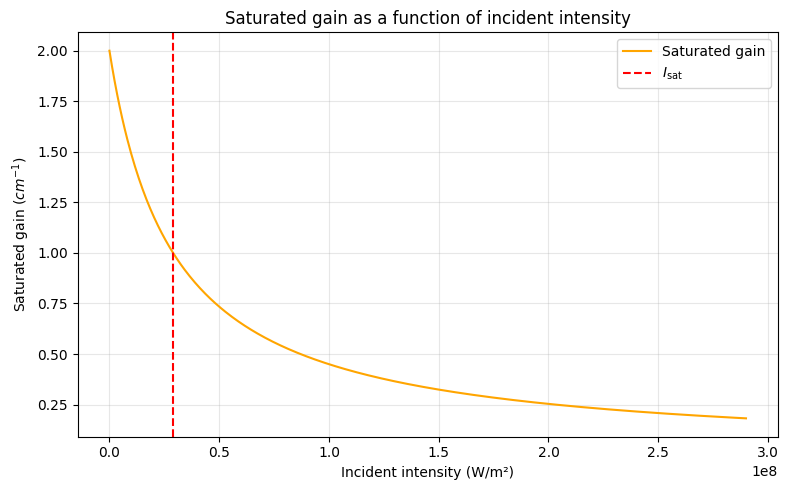
\includegraphics[width=0.9\linewidth]{Images/saturated_gain.png}
        \caption{Saturated gain vs incident intensity}
        \label{fig:saturated_gain}
    \end{figure}

    \item The last request is to compute the total gain of the entire rod in the small-signal regime. In order to do so, we can use the formula:

    \begin{equation}
        G = e^{\gamma_0 L}
    \end{equation}
    Substituting the values for $\gamma_0$ and $L$, we get:
    $$
        G = 2.20 \times 10^4
    $$

\end{enumerate}

These results illustrate the fundamental principles of laser amplifier operation and provide key insights into the trade-offs and considerations in amplifier design, such as pumping power requirements, saturation effects, and the relationship between system parameters and gain performance.


%%%%%%%%%%%%%%%%%%%%%%%%%%%%%%%%%%%%%%%%%%%%%%%%%%%%%%%%%%%%%%%%%%%%%%%%%

\newpage
\section{Vibrational spectrum}
\subsection{Problem statement}
The vibrational frequency in chemical units ($\si{cm^{-1}}$) of a nitrogen molecule is about $f_c = 2360~\si{cm^{-1}}$. Calculate the value of the elastic constant $k_0$ associated with that degree of freedom.

\subsection{Solution}
This problem regards vibrational modes in a nitrogen molecule ($N_2$). In a diatomic molecule, vibrational modes correspond to the periodic motion of the two atoms along the bond axis, oscillating relative to their equilibrium positions due to the restoring force of the chemical bond. This motion can be modeled as a quantum harmonic oscillator, with discrete vibrational energy levels given by:
%
\begin{equation}
    E_v = \left(v + \frac{1}{2}\right)h\nu,
\end{equation}
%
where $v = 0, 1, 2, \dots$ is the vibrational quantum number, $h$ is Planck's constant, and $\nu$ is the fundamental vibrational frequency. The vibrational frequency is determined by the bond's stiffness (force constant $k_0$) and the reduced mass $\mu$ of the two atoms:
%
\begin{equation}
    \label{eq:frequency}
    \nu = \frac{1}{2\pi}\sqrt{\frac{k_0}{\mu}}.
\end{equation}
%
Here, the reduced mass $\mu$ is defined as:
%
\begin{equation}
    \label{eq:reduced_mass}
    \mu = \frac{m_1 m_2}{m_1 + m_2},
\end{equation}
%
where $m_1$ and $m_2$ are the masses of the two atoms in the molecule.

We can leverage this theoretical description to compute the elastic constant $k_0$; first of all, the molecule we are considering is made of two equally weighted atoms, so Equation~\eqref{eq:reduced_mass} reduces to:
%
\begin{equation}
    \label{eq:reduced_mass_2}
    \mu = \frac{m}{2}
\end{equation}
%
Moreover, we need to modify a bit Equation~\eqref{eq:frequency}, as we have the fundamental vibrational frequency in chemical units; taking this and Equation~\eqref{eq:reduced_mass_2} into account, we obtain:
%
\begin{equation}
    f_c= \frac{1}{2\pi c}\sqrt{\frac{k_0}{\mu}} = \frac{1}{2\pi c}\sqrt{\frac{2k_0}{m}} ,
\end{equation}
where $c$ is the speed of light. Now we can simply invert this equation and find a way to compute $k_0$, as all the other data are known:
%
\begin{equation}
    \label{eq:k_0}
    k_0 = \frac{m}{2} (2\pi c f_c)^2 = 2m (\pi c f_c)^2
\end{equation}
%
Considering that for the nitrogen $m = 14.00~\text{au} = 2.32 \times 10^{-26}~\si{\kilo\gram}$, we get:
$$
    k_0 = 2.30~\si{\newton}/\si{\meter}
$$
This value reflects the stiffness of the chemical bond between the two nitrogen atoms, which is directly related to the vibrational frequency of the molecule. The high value of $k_0$ is consistent with the strong triple bond present in $N_2$, a characteristic of its exceptional stability and low reactivity under normal conditions.

\newpage
\section{Heisenberg uncertainty in time}
\subsection{Problem statement}
Take a single-photon state with central $\lambda = 532$~nm that is confined in time to a $\sigma_t = 1$~ns. Discuss the energy spread and the consequences in its spectrum.

\subsection{Solution}
This problem asks to consider a single photon state with a given central wavelength and highly confined in time. It is necessary to take into account the Heisenberg uncertainty principle, which defines a relation between the uncertainty in time and the uncertainty in energy. The time-energy uncertainty relation is expressed as:
%
\begin{equation}
    \label{eq:heisenberg_principle}
    \sigma_E \cdot \sigma_t \geq \frac{\hbar}{2},
\end{equation}
%
where $\sigma_E$ is the energy uncertainty (or spread), $\sigma_t$ is the confinement time, and $\hbar = \frac{h}{2\pi}$ is the reduced Planck constant. From Equation~\eqref{eq:heisenberg_principle}, we observe that the product of the energy uncertainty $\sigma_E$ and the time uncertainty $\sigma_t$ cannot be arbitrarily small; it is bounded from below by $\frac{\hbar}{2}$. This implies that if the temporal confinement of the photon is very tight (small $\sigma_t$), the uncertainty in its energy (or equivalently, its frequency) will increase, and vice versa. Moreover, considering the energy-frequency relationship $E = h\nu$, where $\nu$ is the frequency, the energy uncertainty $\sigma_E$ can be expressed in terms of the frequency uncertainty $\sigma_\nu$:
%
\begin{equation}
    \label{eq:energy_frequency}
    \sigma_E = h \sigma_\nu.
\end{equation}
%
Substituting Equation~\eqref{eq:energy_frequency} into Equation~\eqref{eq:heisenberg_principle}, we obtain the time-frequency uncertainty relation (equivalent to the energy-time relation):
%
\begin{equation}
    \label{eq:time_frequency}
    \sigma_\nu \cdot \sigma_t \geq \frac{1}{4\pi}.
\end{equation}
%
We can use this equation to obtain the minimum frequency spread $\sigma_\nu$ (which is not the actual value of the frequency spread but gives us an order of magnitude of what we are talking about) and consequently the minimum energy spread $\sigma_E$:
$$
    \sigma_\nu \geq \frac{1}{4\pi \sigma_t} = 7.96 \times 10^7~\si{\hertz} \qquad \qquad \qquad \sigma_E = h\sigma_\nu = 5.27 \times 10^{-26}~\si{\joule}
$$ 
In order to make some useful observations, we need to compare the obtained value with the the central frequency $\nu_0$, which, for a single photon with a central wavelength $\lambda_0$, can be determined using the relation:
\begin{equation}
    \label{eq:central_frequency}
    \nu_0 = \frac{c}{\lambda_0},
\end{equation}
where $c$ is the speed of light in vacuum. The corresponding energy of the photon is $E_0 = h\nu_0$. Using the given data we get:
$$
\nu_0 = 5.63 \times 10^{14}~\si{\hertz} \qquad \qquad \qquad E_0 = 3.73 \times 10^{-19}~\si{\joule}
$$
Using a simple error propagation from Equation~\eqref{eq:central_frequency}, we can compute also the spectral bandwidth (which represents the wavelength uncertainty):
%
$$
    \Delta \lambda = \frac{\lambda^2\Delta\nu}{c} \geq \frac{\lambda^2\sigma_\nu}{c} \geq 7.51 \times 10^{-14}~\si{\meter}
$$
\newpage
Observing the results, we can draw the following conclusions:
\begin{itemize}
    \item The minimum frequency uncertainty $\sigma_\nu$ is much smaller than the central frequency $\nu_0$. Specifically, the ratio $\sigma_\nu / \nu_0 \approx 1.41 \times 10^{-7}$ indicates that the uncertainty is negligible compared to the central frequency. This reflects on the spectral bandwidth $\Delta \lambda$, which is extremely narrow, with a value on the order of $10^{-14}~\si{\meter}$. Thus, we can conclude that the photon is well-defined in its spectral domain despite its temporal confinement.
    
    \item Similarly, the minimum energy uncertainty $\sigma_E$ is significantly smaller than the photon energy $E_0$. The ratio $\sigma_E / E_0 \approx 1.41 \times 10^{-7}$ supports the notion that the photon remains well-characterized energetically, even under the constraints of temporal confinement.
\end{itemize}

These results highlight the interplay between time and frequency domains for a single photon. The Heisenberg uncertainty principle enforces a trade-off, but in this case, the photon is designed to balance these constraints effectively. The extreme localization in time leads to only a modest increase in spectral spread, demonstrating the precision achievable even under strict temporal confinement.

%%%%%%%%%%%%%%%%%%%%%%%%%%%%%%%%%%%%%%%%%%%%%%%%%%%%%%%%%%%%%%%%%%%%%%%%%


\end{document}
